\documentclass[a4paper,12pt,titlepage]{scrartcl}

\usepackage[utf8]{inputenc}

\usepackage{hyperref}
\hypersetup{
    colorlinks=true,
    linkcolor=black,
    filecolor=magenta,      
    urlcolor=blue,
}

\usepackage{graphicx}
\graphicspath{ {./images/} }

\usepackage{fancyhdr}
\usepackage{lastpage}

\usepackage{listings}

\usepackage{float}

\pagestyle{fancy}
\fancyhf{}

\rfoot{Page \thepage \hspace{1pt} of \pageref{LastPage}}

\title{\textbf{KiloGuide}\\User Guide}
\titlehead{\centering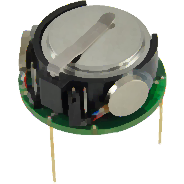
\includegraphics{kilogo.png}}
\author{Simon Lejoly}
\date{May 2021}

\begin{document}

\maketitle

\newpage

\tableofcontents

\newpage

\section{Overview}

\textbf{KiloGuide} is a simple guide about \href{https://kilobotics.com}{kilobots}. \emph{Kilobots} are small physical robots designed by the University of Harvard and commercialized by the K-Team, commonly used to study swarm robotics. KiloGuide explains how to perform various tasks such as calibration or code compilation and provides multiple small projects to illustrate how coding for kilobots is done.

\section{Features}

KiloGuide is divided in two sections: \textbf{guides} and \textbf{tutorials}.

The \textbf{guides} aim to explain you basic kilobots operations, such as "transferring code to a kilobot", "calibrating kilobots" or "using Kilo-GUI".

The \textbf{tutorials} focus on the implementation part. With tutorials, you will learn how to code for kilobots through easy and diverse projects.

\subsection{Guides}

KiloGuide currently contains 5 guides: 

\subsubsection{Getting started with kilobots}

Learn how to turn your kilobots on and off. Discover the components of a kilobot and what it can do with them. Know how to calibrate your kilobots.

\subsubsection{Coding for kilobots}

Learn the basics of robot programming, which language and which code templates are used to write programs for kilobots.

\subsubsection{Compile your code}

Learn how to convert your code into an executable file, that will be read by your kilobots.

\subsubsection{Transfer and run your program}

Learn how to transfer the executable file into your kilobots, start, pause and stop the program.

\subsubsection{Use the debug feature}

Learn how to use the simple debug feature with kilobots, to know what is not working in your programs.

\subsection{Tutorials}

KiloGuide currently contains 5 tutorials:

\subsubsection{Race Around the World}

Learn the basics of robot programming with one single kilobot. Write a simple program to turn on its LED and make it move along a race track.

\subsubsection{Full Metal Kilobot}

Get into a more complex program and use communication between two kilobots in a creative way. One of the kilobots is the instructor, yelling orders to the rookie, which must then execute them... with more or less precision.

\subsubsection{King-o-bot's Games}

In this tutorial inspired by medieval knight tournaments, the kilobots must fight in duel, going one toward the other at astounding speeds. The first to freak out loses and shall not be King-o-bot's great champion!

\subsubsection{Morphogenetics}

In the body of living creatures, a cell can sometimes approximate its distance to another cell by analysing the neighbouring concentration of chemicals produced by that cell. Let's put this idea in practice with kilobots!

\subsubsection{Rush Hour}

In this tutorial, a lot of kilobots are placed in a limited space. As they move around randomly, they must display different colors depending on the number of kilobots they detect around them. The goal is to obtain some heat-map of the kilobot concentrations at a high scale.

\section{Access / Download}

\subsection{Access from the Internet}

You can easily access KiloGuide online following \href{https://simlej18.github.io/KiloGuide/}{this link}.

\subsection{Download}

If you want to have access to KiloGuide offline, you may download it from \href{https://www.mediafire.com/file/olqogopejhlbe3z/KiloGuide.zip/file}{this website}.

\section{Getting started}

\subsection{Getting started from the online version}

If you followed the link above, you should already see the homepage of KiloGuide. 

\subsection{Getting started from the downloaded version}

The downloaded file should be a zip archive. Un-zip it and enter the KiloGuide directory. You should find a file named \emph{"index.html"}. Open this file in your Internet browser. You should now see KiloGuide's homepage!

\subsection{Getting started with kilobots}

If you have never used kilobots before, the \emph{"Getting started"} guide is a good starting point. You can access it from the navigation bar (see below).

\subsection{Navigate through the guide}

\begin{figure}[H]
  \makebox[\textwidth][c]{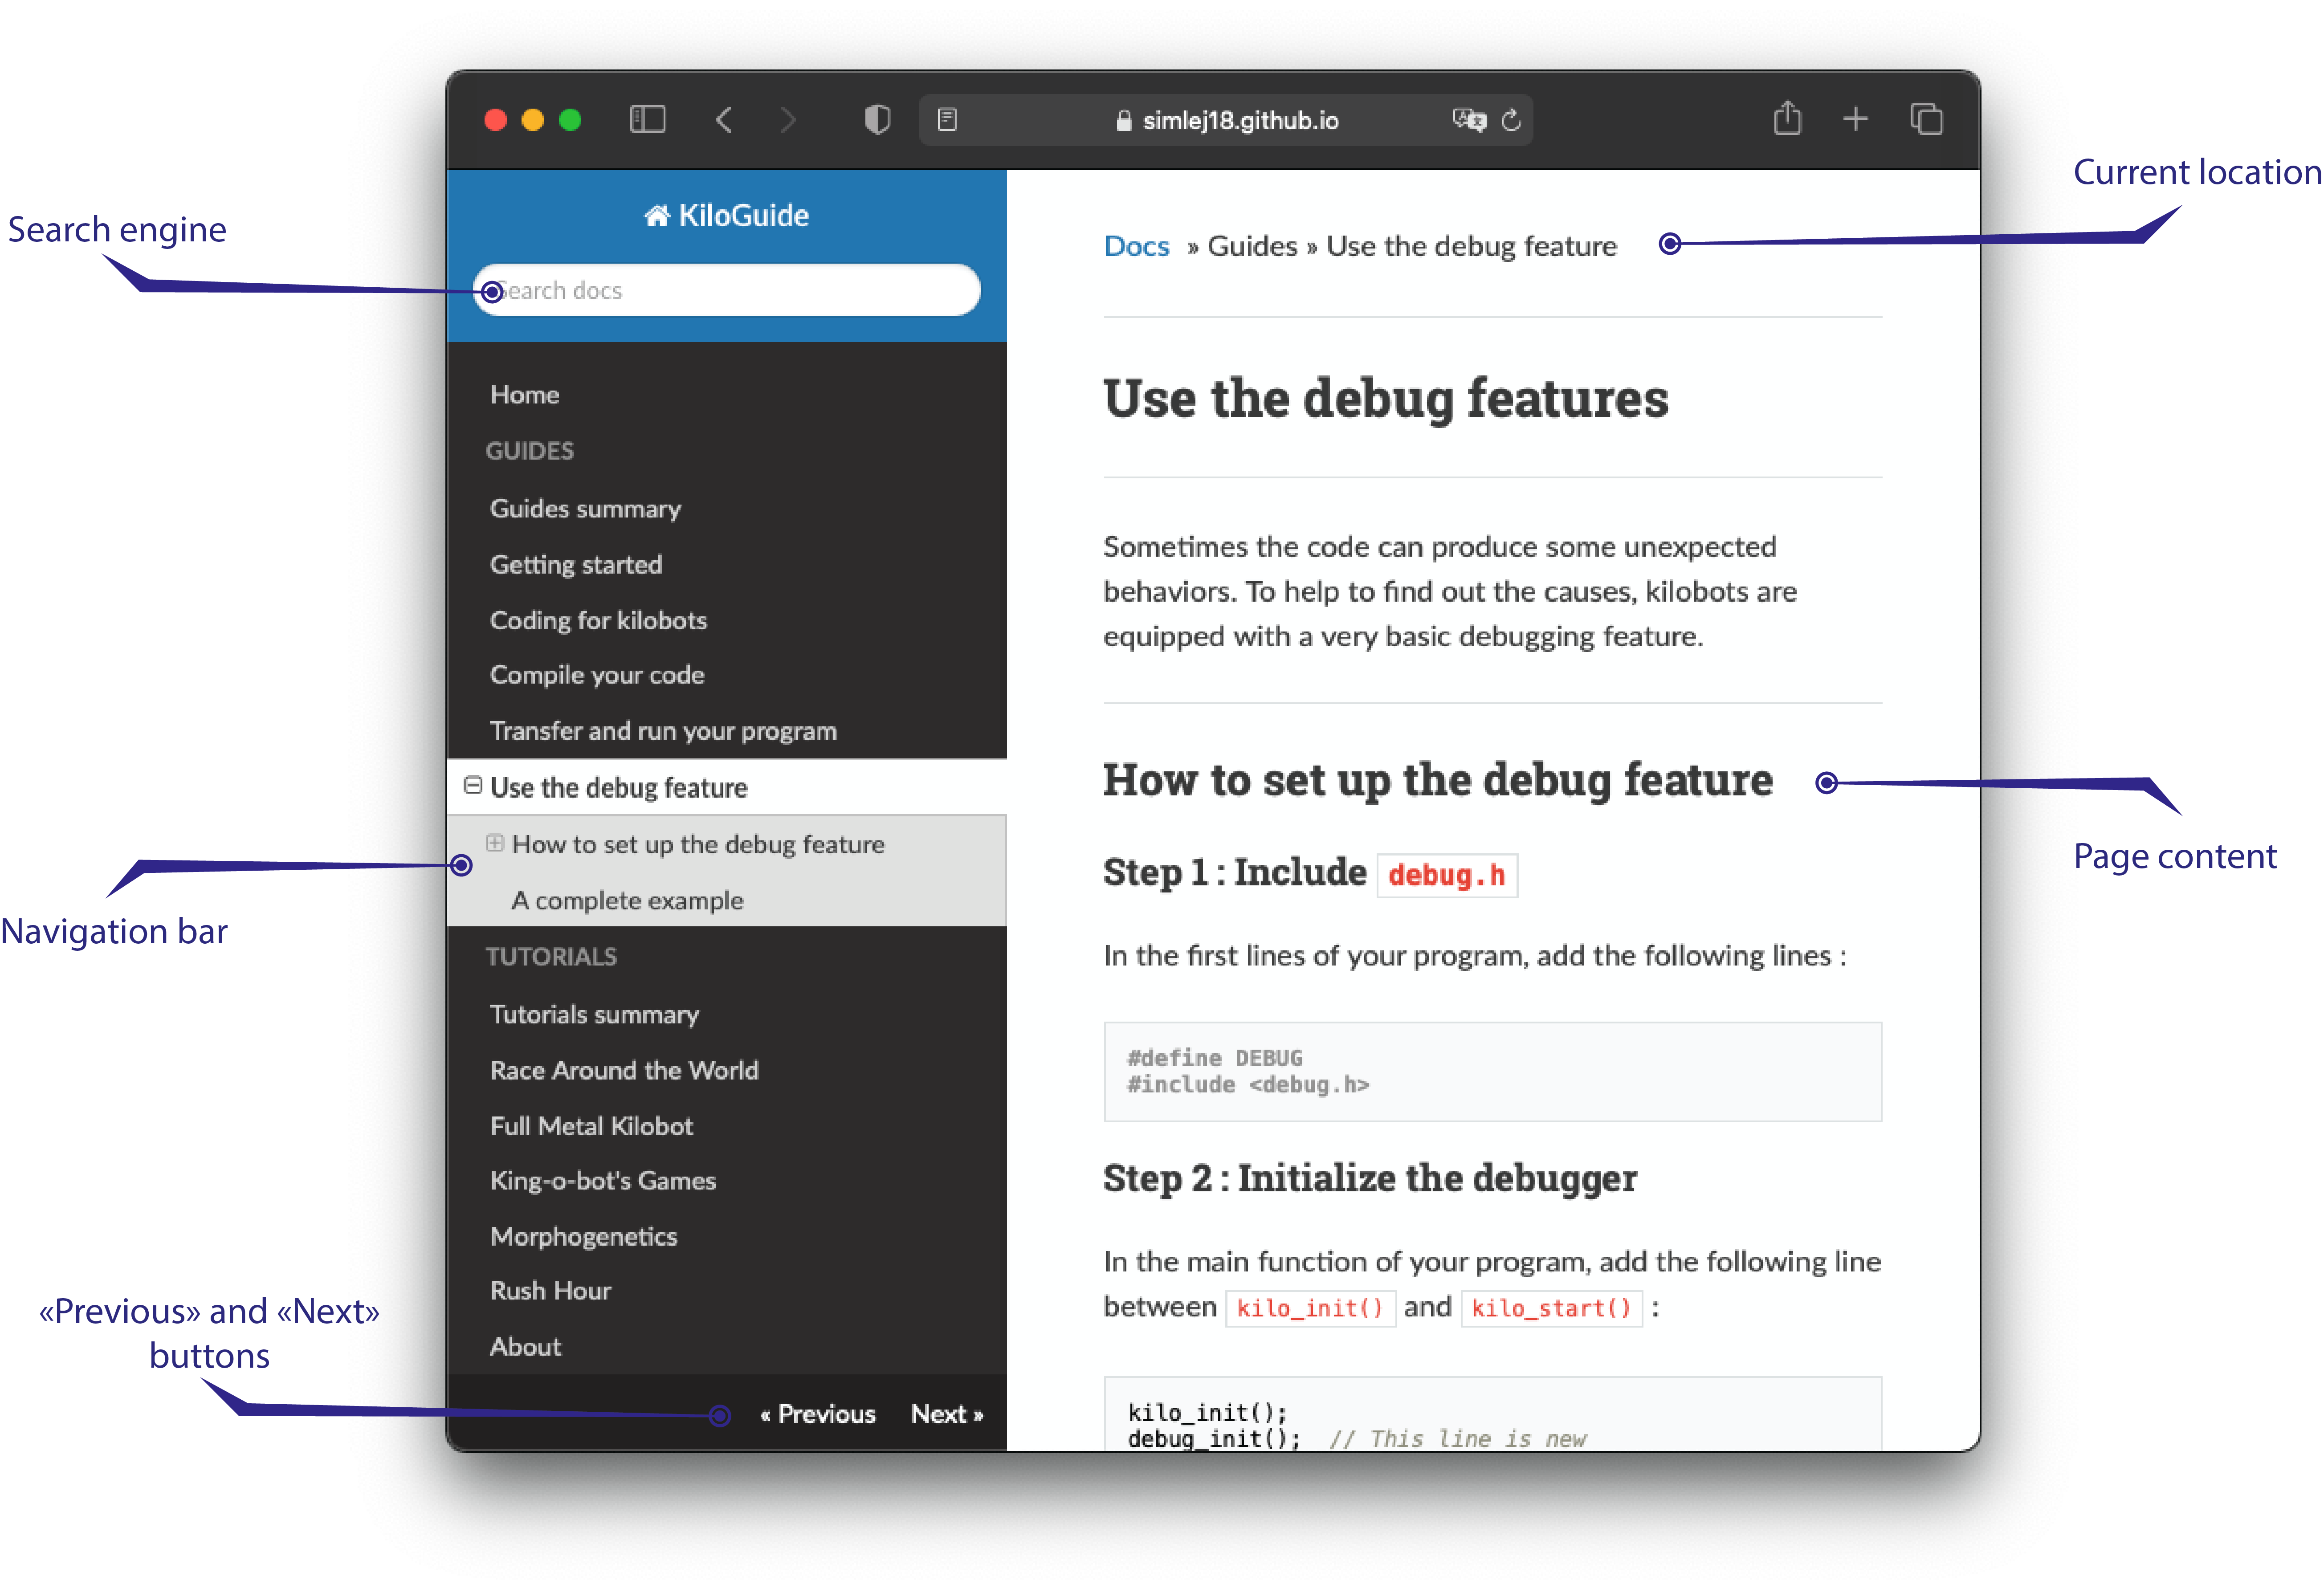
\includegraphics[scale=0.68]{expl.png}}
\end{figure}

\subsubsection{Navigation bar}

On the left side of the website you will find the navigation bar. It is composed of two pages (\emph{"Home"} and \emph{"About"}) and two categories (\emph{"Guides"} and \emph{"tutorials"}), each containing 6 other pages.

You can access each page by clicking on it. Note that clicking on a category will lead you nowhere. However, the \emph{"Guide summary"} and \emph{"Tutorials summary"} pages are meant to give you an overview of all the guides / tutorials.

\subsubsection{"Next" and "Previous" buttons}

If you wish to read each page of the guide one after the other, you should use the \emph{"Next"} and \emph{"Previous"} buttons. You can access these buttons at the bottom of the navigation bar. You will also find them at the end of each page.

\begin{center}

\includegraphics[scale=0.6]{previous&next.png}
\end{center}

\subsubsection{Search engine}

You may want to look for information about one specific aspect of kilobots. To help you find them, KiloGuide is equipped with a \emph{search engine}. You can access this search engine at the top of the navigation bar.

Once you have written what you are looking for, press "enter" to be redirected to the \emph{result page}. This page displays all the sections of KiloGuide related to the keywords you have entered. 

\begin{center}
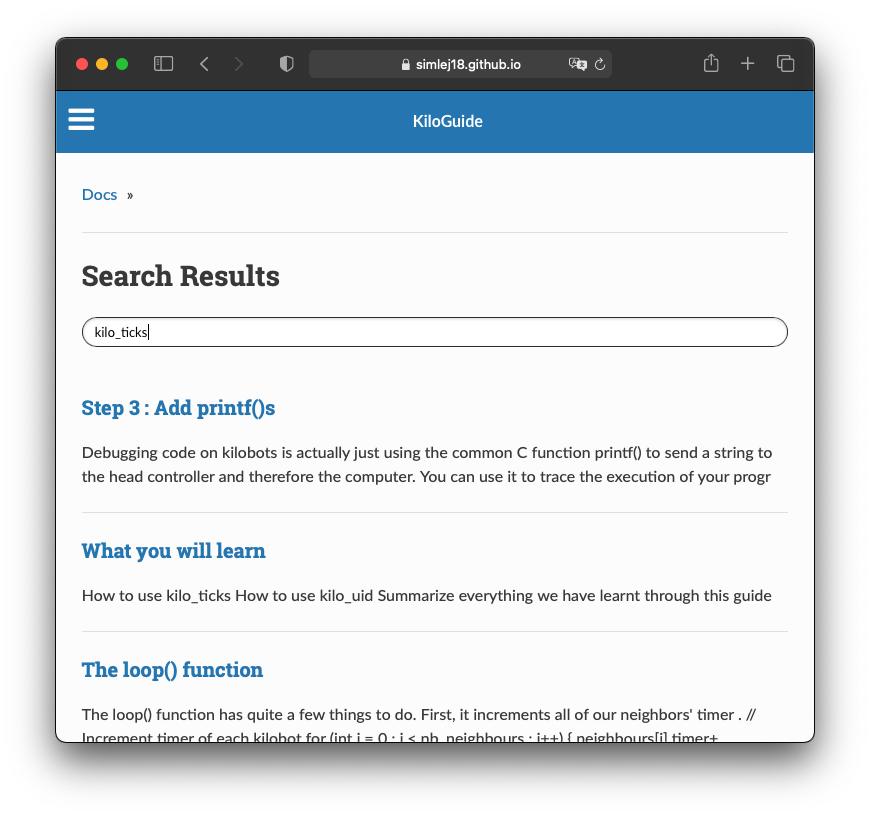
\includegraphics[scale=0.3]{kilosearch.png}
\end{center}

\section{Troubleshooting}

Here are the most common problems that can occur when using KiloGuide:\\

\textbf{The zip archive cannot be un-zipped}

A problem might have happened during the download process. Download KiloGuide a second time and try again. Make sure that your internet browser and operating system are up-to-date and that your access to the Internet is stable.\\

\textbf{The navigation bar does not appear}

When the window is too thin (on mobile devices, for example), KiloGuide hides the navigation bar. You can access it either by expanding your window horizontally or by clicking the little drawer icon 
\includegraphics[height=11px]{drawer.png} in the top-left corner.\\

\textbf{Some parts of the guide seem too obscure / complicated}

KiloGuide is fully-independant from the team designing the kilobot and its programming library. If you have troubles with the kilobot environment, consider visiting the sources listed in the "Resources and troubleshooting" section of KiloGuide's homepage.

\section{FAQ}

Here are some frequently asked questions about KiloGuide:\\

\textbf{I spotted a mistake in KiloGuide. How can I report it?}

You can report any mistake in the "issues" section of \href{https://github.com/SimLej18/KiloGuide}{KiloGuide's GitHub repository}. Before posting an issue, make sure that it was not already spotted by another user. 

\emph{Note that KiloGuide comes with no guarantee in terms of maintenance and that your issue may remain unsolved.}\\

\textbf{I want to contribute to the KiloGuide project. How can I do so?}

You can contribute to the KiloGuide project by submitting a pull request in the "pull requests" section of \href{https://github.com/SimLej18/KiloGuide}{KiloGuide's GitHub repository}. 

Before doing so, you might want to understand how KiloGuide is implemented. You will find useful information in \emph{KiloGuide's developper guide}, which is available in the repository.

\emph{Note that KiloGuide comes with no guarantee in terms of maintenance and that your pull request may not be approved or even reviewed.}\\

\textbf{Are there differences between the online version and the downloadable version of KiloGuide?}

To this day, both versions are completely identical. However, if KiloGuide was to receive an update, previous downloaded copies would be deprecated and should be re-downloaded. The online version on the other hand, will always stay up-to-date.

\section{Contact}

KiloGuide and its user guide were written by \emph{Simon Lejoly} (\href{mailto:simonlejoly@icloud.com}{simonlejoly@icloud.com}) and are part of a project conducted by the \emph{University of Namur}.

Some of the content of this user guide, including images, may be subject to copyright.\\\\

\begin{center}

\includegraphics[scale=0.3]{unamur.png}
\end{center}

\end{document}
